\documentclass[a4paper,10pt]{article}
\usepackage{epsfig}
\usepackage{latexsym}
\usepackage{amssymb}
\usepackage{amsmath}
\usepackage{amsfonts}
\usepackage{lscape}
\usepackage{color}
\usepackage{vmargin}
\usepackage{url}
\usepackage{bbm}
%\usepackage{bbold}

\usepackage{listings}
\lstset{
         numbers=left,               
         stepnumber=1,                     
         numberfirstline=true,
				 firstnumber=1
 }


\setpapersize{A4}

\newcommand{\E}{\mathbb{E}}                 %The expected value function.
\newcommand{\Var}{\mathbb{V}{\rm ar}}       %The variance function.
\newcommand{\Cov}{\mathbb{C}{\rm ov}}       %The covariance function.
\newcommand{\SDev}{\mathbb{SD}{\rm ev}}     %The standard deviation function.
\newcommand{\Corr}{\mathbb{C}{\rm orr}}     %The correlation function.
\newcommand{\CVar}{\mathbb{CV}{\rm ar}}     %The coefficient of variation.
\renewcommand{\P}{\mathbb{P}}               %The probability measure P.
\newcommand{\Q}{\mathbb{Q}}                 %The probability measure Q.
\newcommand{\pdone}[2]{\ensuremath{\frac{\partial #1}{\partial #2}}}
                                            %First order partial derivatives.

\begin{document}
\begin{center}
{\bf \LARGE QuantSA\\}
\normalsize A free, easy to use quant library for SA
\end{center}

\section{Introduction}

%%%%%%%%%%%%%%%%%%%%%%%%%%%%%%%%%%%%%%%%%%%%%%%%%%%%%%%%%%%%%%%%%%%%%%%%%%%%%%%
%%% Library Philosophy
%%%%%%%%%%%%%%%%%%%%%%%%%%%%%%%%%%%%%%%%%%%%%%%%%%%%%%%%%%%%%%%%%%%%%%%%%%%%%%%
\section{Library Philosophy}
Pre-crisis quantitative analysis was often about hand solving for the present value of a product under different proposed dynamics for what were deemed relevant underlying market factors.  Currently the focus is moving more towards valuing more diverse portfolios and then modelling additional cashflows that arise at a portfolio level for example:
\begin{itemize}
	\item flows in default
	\item flows from funding activities
	\item flows from margin placement and receipt, both initial and variational
	\item and many others
\end{itemize}
These additional flows are often not specified in the confirmation contract between the counterparties but are rather contained in the ISDA master agreements, agreements with exchanges, internal agreements and agreements with regulators.  This library attempts to separate the implementation of modelling these features into separate problem domains that can be solved, or at least improves upon, in near isolation.  This means that if the quant needs to answer questions in one domain they do not need to implement features in all the rest.

\textbf{Example 1}: Imagine we had a library that could value all the products that we cared about could be valued but the models contained no correlation between bonds and equities.  It then emerges bonds and equities are highly correlated.  The addition of the correlation should be possible without changing the products and valuation adjustments.

\textbf{Example 2}: The regulators propose a new capital requirement that is a function of the value of your portfolio and some sensitivities of your portfolio to benchmark instruments.  You want to know some statistics about the capital utilization over the next year, such as the expected amount or some high percentile to measure how high the utilization may become.  You should be able to solve this by simply implementing the capital rule applying it to an already existent simulation of values and sensitivities.

%%%%%%%%%%%%%%%%%%%%%%%%%%%%%%%%%%%%%%%%%%%%%%%%%%%%%%%%%%%%%%%%%%%%%%%%%%%%%%%
%%% Parts of QuantSA
%%%%%%%%%%%%%%%%%%%%%%%%%%%%%%%%%%%%%%%%%%%%%%%%%%%%%%%%%%%%%%%%%%%%%%%%%%%%%%%
\section{Parts of QuantSA}
At the top level there are two parts to QuantSA:
\begin{itemize}
	\item The Excel layer
	\item The library
\end{itemize}
The library is then also split into parts that represent different problem domains:
\begin{enumerate}
	\item Products
	\item Market factor simulators
	\item A regression and machine learning layer
	\item Higher order cashflow modelling
\end{enumerate}
There is also supporting functionality (e.g. calibrators, formulas, interpolators, date functions, closed form approximations, etc) that is not a competent of the main architecture and some freedom is possible in organizing this.  	

The four main parts have well defined interfaces between them and the addition of features in any one of them will be available to any others.  For example a better regression model for getting forward valuation will work for all products or a new capital model in the higher order layer will work on any products or simulations.


%%%%%%%%%%%%%%%%%%%%%%%%%%%%%%%%%%%%%%%%%%%%%%%%%%%%%%%%%%%%%%%%%%%%%%%%%%%%%%%
%%% Market Setup
%%%%%%%%%%%%%%%%%%%%%%%%%%%%%%%%%%%%%%%%%%%%%%%%%%%%%%%%%%%%%%%%%%%%%%%%%%%%%%%
\section{Market Setup}
The general framework in QuantSA is very similar to that described in in Cesari \textit{et al} (2010) \cite{cesari2010modelling} except that we have removed the portfolio aggregation language. In its place we use a set of $K$ market observables.  The basis of this is that any contractually agreed cashflow between counterparties is defined unambiguously in terms of observed index values.  Obvious exceptions to this is a claim in default or a transfer of collateral.  These latter two exceptions are based on essentially subjective assessments of value and have a dispute mechanism.  The cashflow types that are not completely unambiguous are handled in the higher order cashflow modelling part of QuantSA.  An intermediate type of cashflow originates from decisions made by one of the counterparties, the main example of this is an exercise decision, while this is not objectively known, we can however assume that the counterparty acts rationally and maximizes their value.

The $K$ market observables are labeled $S_1,...S_K$ and can be observed at a finite number of days, possibly before any given valuation date.  The date on which a valuation takes place is labeled $t_0$. 

The objective flows on any product or portfolio take place at fixed times and are calculated as functions of the $K$ market observables.  In general if there is a cashflow at $u_i$ it will depend on market observables at times on or before $u_i$
\begin{equation}
X_i = f(S_{j_0}(v_{k_0}), S_{j_1}(v_{k_1}), ...) 
\end{equation}
with $(j_l, k_l)$ in some set $\mathcal{J}(u_i)$ that depends on the product and $u_i$.

The value of any product at $t_0$ is then:
\begin{equation}
V(t_0) = \E^\Q\left[ \sum_{u_i>t_0}{\frac{S_{xn}(u_i)X_i}{N(u_i)}} \right]
\end{equation}
Where $N(u_i)$ is the numeraire in the value currency and $S_{xn}$ is that market observable that converts units of the cashflow currency into units of the numeraire currency, i.e. the exchange rate.
Any product without optionality can then be represented by the set of random variables and the times at which the cashflows represented by the random variables take place:
\begin{equation}
P = \left\{ \left(X_1, u_1\right), ..., \left(X_M, u_M\right) \right\}
\end{equation}

\subsection{Monte Carlo}
We assume that our economy is described by some probability space $(\Omega, \mathcal{F}, \Q)$ with maximum time $T$.  In that space we have a vector vector stochastic process $\textbf{W}(t)$ and the filtration $\mathcal{F}(t)$ generated by $\textbf{W}(t)$.  The $S$s and $N$ are then all functions of $\textbf{W}$.

Different models are then different definitions of $\textbf{W}$ and different functions to create the asset prices.  
This allows us to value any product in any model using Monte Carlo.

\subsection{Forward Value}
If we require the forward value at time $t_i > t_0$ we need to evaluate
\begin{equation}
V(t_i) = N(t_i)\E^\Q\left[ \sum_{u_i>t_i}{\frac{S_{xn}(u_i)X_i}{N(u_i)}} \middle| \mathcal{F}(t_i) \right]
\label{eq:fwdvalue1}
\end{equation}
Note that $V(t_0)$ is not random since all states of the world agree up to $t_0$ the time we are at when we fit the model and perform the valuation, but if $t_i>t_0$ then $V(t_i)$ is random and will be a function of the world observed up to $t_i$
This could be evaluated with another Monte Carlo simulation beyond $t_i$ for each state of the world observed up to $t_i$ but as discussed in many sources [...] this is expensive.  So we assume that $\textbf{W}$ is Markov and note (see Shreve \cite{Shreve} Def 2.3.6) that 
\begin{equation}
V(t_i) = g(t_t, \textbf{W}(t_i))
\label{eq:regress}
\end{equation}
Longstaff and Schwartz \cite{Longstaff01valuingamerican} describe how to use regression to estimate this function $g$ given realizations of $\sum_{u_i>t_i}{\frac{S_{xn}(u_i)X_i}{N(u_i)}}$, an example of this can be seen in Figure \ref{fig:ConditionalExpectationEx1}.

\begin{figure}
	\centering
		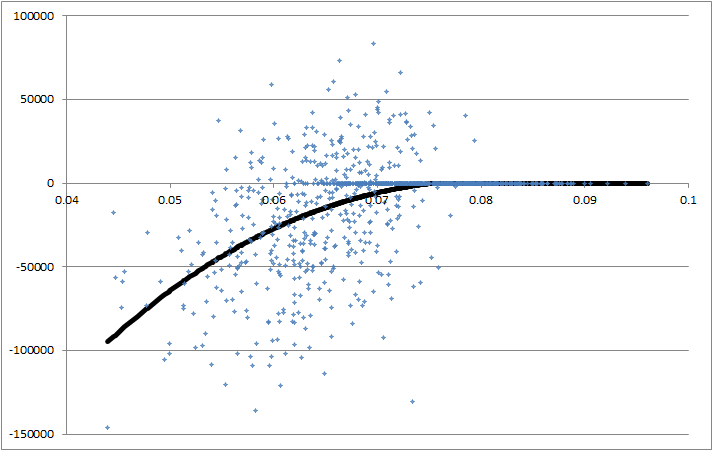
\includegraphics[width=100mm]{ConditionalExpectationEx1.png}
	\caption{Simulated cashflows and estimated conditional expectation.}	
	\label{fig:ConditionalExpectationEx1}
\end{figure}

\subsection{Optionality}
When one of the counterparties has a decision to make, it is always between a finite set of alternatives, and each alternative must either define unambiguous cashflows or a set of cashflows that themselves have some optionality in them.

A general product with a finite possible set of exercise dates can be represented as the cashflows that will be received until exercise and the product/set of cashflows that will be exercised into.
\begin{equation}
O = P_{noex} \text{ and } \left\{ \left(Q_1, e_1\right), ..., \left(Q_M, e_M\right) \right\}
\end{equation}
Where the $Q_i$ are the products that will be exercised into if the optimal stopping time is equal to $e_i$.  For now assume that all the $Q$s are no exercise products, then using the above discussion on forward valuation we can produce at any exercise time $e_i$ simulations of $v_P(j)$ and $v_Q(j)$ the values of the no exercise and post exercise products on each path.

The value of a product with optionality is given by:
\begin{equation}
V^{optimal}(t_0) = \E^\Q\left[ \sum_{u_i>t_0}\mathbbm{1}_{u_i\leq\tau}{\frac{S_{xn}(u_i)X_i}{N(u_i)}}  + 
\mathbbm{1}_{\tau=e1}\sum_{u_i^{Q_1}>t_0, e_1}{\frac{S_{xn}(u_i^{Q_1})X^{Q_1}_i}{N(u^{Q_1}_i)}} + ...
\right]
\end{equation}
and 
\begin{equation}
V^{optimal}(t_i) = \E^\Q\left[ \sum_{u_i>t_i}\mathbbm{1}_{u_i\leq\tau}{\frac{S_{xn}(u_i)X_i}{N(u_i)}}  + 
\mathbbm{1}_{\tau=e1}\sum_{u_i^{Q_i}>t_i,e_1}{\frac{S_{xn}(u_i^Q)X^{Q_1}_i}{N(u^{Q_1}_i)}} + ...
\middle| \mathcal{F}(t_i)\right]
\label{eq:fwdvalue2}
\end{equation}
for $\tau$ the optimal $\mathcal{F}(t)$ measurable stopping time.

We need an algorithm to construct $\tau$, we do something similar to what is done in \cite{cesari2010modelling} and \cite{AntonovEtAl2015}.  On each path set to optimal exercise time $\tau_j$ to $\infty$.  At the last exercise time $e_M$ the owner of the option will exercise on paths $j$ where $v_{Q_M}(j)>v_P(j)$.  On the paths where this happens we update $\tau_j$ to $e_M$.

We then know $\tau$ conditioned on $\tau>e_{M-1}$ so we can calculate $V^{optimal}(e_{M-1}+\epsilon)$, the pathwise stopping time is then updated to $e_{M-1}$ on the paths where $v_{Q_M}(j) > v^{optimal}(j)(e_{M-1}+\epsilon)$.  This continues back through all the exercise dates.

If it happened that one of the exercise products itself has optionality then the stopping times on that product would need to be solved first, and the above routine can be applied recursively with the deepest/first evaluated pass valuing a product that only depends on other products without exercise.

\subsection{General forward values}
The section on optionality is only applied to obtain the optimal stopping times for each product that contains some optionality.  Antonov \textit{et al} \cite{AntonovEtAl2015} perform the forward valuations and optimal exercise rules in a single backward pass.  We elect to do the optionality in a backward pass and then store these stopping times.  The evaluation of Equations \ref{eq:fwdvalue1} and \ref{eq:fwdvalue2} via Equation \ref{eq:regress} can then be done out of sequence for the whole portfolio on multiple threads.


%%%%%%%%%%%%%%%%%%%%%%%%%%%%%%%%%%%%%%%%%%%%%%%%%%%%%%%%%%%%%%%%%%%%%%%%%%%%%%%
%%% Further work
%%%%%%%%%%%%%%%%%%%%%%%%%%%%%%%%%%%%%%%%%%%%%%%%%%%%%%%%%%%%%%%%%%%%%%%%%%%%%%%
\section{Further work}
What if the option on a contract will depend on higher order cashflows.  For example perhaps a counterparty has the option to exercise into a physical swap, the swap on its own is slightly out of the money but the addition of that swap the the portfolio would decrease capital or margin requirements making the exercise decision optimal.  Or the swap could be in the money at the exercise date on a credit free basis but when it is adjusted for the counterparty risk it has a negative fair value.


\bibliographystyle{plain}
\bibliography{publications}
\end{document}

